\documentclass{article}

% Language setting
% Replace `english' with e.g. `spanish' to change the document language
\usepackage[german]{babel}

% Set page size and margins
% Replace `letterpaper' with `a4paper' for UK/EU standard size
\usepackage[a4paper]{geometry}

% Useful packages
\usepackage{amsmath}
\usepackage{graphicx}
\usepackage[colorlinks=true, allcolors=blue]{hyperref}
\usepackage{float}
\usepackage{multicol}
\usepackage{xcolor}

\setlength{\columnseprule}{0.5pt}
\def\columnseprulecolor{\color{blue}}
\title{Wissensicherung}
\author{Asha Schwegler}

\begin{document}
\maketitle

\tableofcontents

\pagebreak

\section{LE01}
\subsection{Was ist Software Engineering?}

\begin{itemize}
 \item Herstellung oder Entwicklung 
von Software,  Organisation und Modellierung der zugehörigen Datenstrukturen und 
dem Betrieb von Softwaresystemen. 
 \item Anhand eines strukturierten (Projekt-)Planes. (Schritte, Phasen, Meilensteine)
 \item Schritte während Entw.Prozess eng miteinander verzahnt.
\end{itemize}

\subsection{Was für Prozesse bzw. Disziplinen können im Software Engineering unterschieden werden?}

\paragraph{Kernprozesse\\}
\begin{itemize}
	\item Anforderungserhebung
	\item Systemdesign/technische Konzeption
	\item Implementierung
	\item Softwaretest
	\item Softwareeinführung
	\item Wartung/Pflege
\end{itemize}

\paragraph{Unterstützungsprozesse\\}
\begin{itemize}
	\item Projektmanagement
	\item Qualitätsmanagement
	\item Risikomanagement
\end{itemize}

\subsection{Was sind die Charakteristiken eines iterativ-inkrementellen Softwarenentwicklungsprozesses?}
\begin{itemize}
	\item Abwicklung in Iterationen
	\item Inkrement = In jeder Iteration ein Stück SW entwickelt
	\item Ziele sind Risiko-getrieben
	\item Iterationsreviews mit Learnings für nächste Iteration
\end{itemize}



\subsection{Warum wird im Software Engineering modelliert und was für Modelle werden erstellt?}
Analyse- und Designentwürfe : diskutieren, abstimmen, dokumentieren und kommunizieren. \\
\begin{itemize}
	\item Verstehen eines Gebildes
	\item  Kommunizieren
	\item Gedankliches Hilfsmittel
	\item Kritisieren
	\item Experimentieren
	\item Aufstellen und Prüfen von Hypothesen
	\item in OOP: 
	\begin{itemize}
		\item Statische Modelle:
		\begin{itemize}
			\item Klassen und Assoziationen
		\end{itemize}
		\item Dynamische Modelle:
		\begin{itemize}
			\item Abläufe und Verhalten
		\end{itemize}
	\end{itemize}
\end{itemize}



\subsection{Welche Artefakte werden in der Anforderungsanalyse erstellt und wozu werden sie gebraucht?}

\begin{itemize}
	\item Systemabgrenzung und Systemkontextdiagramm
	\item Use-Case-Modell und UI-Sketches
	\item Qualitätsanforderungen und Randbedingungen
	\item Domänenmodell
\end{itemize}




\section{LE02}

\subsection{Was ist Usability und Usability-Engineering?}

\textbf{Usability:} Die Effektivität, Effizienz und Zufriedenheit mit der die adressierten Benutzer ihre Ziele erreichen in ihren spezifischen Kontexten.\\
\textbf{Usability Engineering:} Software entwickeln, die die drei Anforderungen von Usability erfüllen.


\subsection{Was ist Usability-Engineering und was sind seine Ziele?}
\begin{itemize}
	\item Usability-Engineering = Software-Ergonomie
	\item Ziel: SW-Produkte entwickeln, die effektiv, effizient und zufriedenstellend sind.
\end{itemize}


\subsection{Welche 7 Usability-Aspekte sind gemäss ISO EN 9241-110 wichtig und was fordern sie?}

\begin{enumerate}
	\item Aufgabenangemessenheit
	\begin{itemize}
		\item Aufwand im Vergleich zu Aufgaben und Ziele sollte angemessen sein.
	\end{itemize}
	\item Selbstbeschreibungsfähigkeit
		\begin{itemize}
		\item Wissen wo in der SW man ist und was man tun muss/kann und was das System tut.
	\end{itemize}
	\item Kontrolle
		\begin{itemize}
		\item Kontrolle über Interaktion mit System haben.
	\end{itemize}
	\item Erwartungskonformität
		\begin{itemize}
		\item Funktionalität
		\item Interaktion
		\item Design
		\item Struktur
		\item Ansprechen der Komplexität
	\end{itemize}
	\item Fehlertoleranz
		\begin{itemize}
		\item Fehler vermeiden
		\item Fehler und Ursache erkennen
		\item Fehler korrigieren
	\end{itemize}
	\item Inidividualisierbarkeit
		\begin{itemize}
		\item Anpassbar auf Bedürfnisse (Laien, Experten, Benutzer mit besondeen Bedürfnisse)
	\end{itemize}
	\item Lernförderlichkeit
		\begin{itemize}
		\item Informationen über unterliegende Konzepte, Reglen, Verfahren und neue Funktionalitäten/Interaktionsmöglichkeiten
	\end{itemize}
\end{enumerate}



\subsection{Was sind die wichtigsten Artefakte aus dem UCD-Prozess und was beschreiben sie?}


\begin{enumerate}
	\item Personas
	\begin{itemize}
		\item Repräsentiert Benutzergruppe (fiktive Beschreibung)
	\end{itemize}
	
	\item Usage-Szenarien
	\begin{itemize}
		\item Aktuelle Situation, Beschreibung wie Persona BESTEHENDES System benutzt um Aufgabe zu lösen.
	\end{itemize}
	
	\item Kontextszenario
	\begin{itemize}
		\item Zukünftige Situation, Beschreibt wie Persona zukünftiges im Idealfall benutzen wird.
	\end{itemize}
	
	\item Storyboard
	\begin{itemize}
		\item Visualisierung vom Kontextszenario
	\end{itemize}
	
	\item Mentales Modell
	\begin{itemize}
		\item Domänenmodell (Vorstellung Benutzers über Problemdomäne)
	\end{itemize}
	
	\item Wireframes (Interaktionsprototypen)
	\begin{itemize}
		\item Demonstration der Interaktion mit dem System
	\end{itemize}
	
	\item Stakeholder Map
	\begin{itemize}
		\item Direkte Akteure und weitere Stakeholder, die interessiert oder betroffen sind vom SW-Produkt
	\end{itemize}
	
	\item Service Blueprint / Geschäftsprozessmodell
	\begin{itemize}
		\item Darstellung logischen Schritte Service kunden, Service-Providers, und über welche Kanäle interagiert wird.
	\end{itemize}
\end{enumerate}




\section{LE03}


\subsection{Fully-dressed UCs
}

\paragraph{UC01: Teilbestellung erfassen\\}

\subparagraph{Umfang: } Swift4Restaurants-Anwendung
\subparagraph{Ebene: } Anwenderziel
\subparagraph{Primärakteur: } Servierperson
\subparagraph{Stakeholder und Interessen:\\}
\begin{itemize}
	\item Servierperson, anderes Servierpersonal:
	\begin{itemize}
		\item Schnelle, genaue und flexible Erfassung der Bestellwünsche
	\end{itemize}
	\item Gast:
	\begin{itemize}
		\item Schnelle und genaue Erfassung seines Bestellwunsches
		\item Nicht mehr bezahlen als konsumiert
	\end{itemize}
	\item Koch:
	\begin{itemize}
		\item Genaue Erfassung des Bestellwunsches
	\end{itemize}
	\item Gastwirt:
	\begin{itemize}
		\item Schnelle und genaue Erfassung Bestellwunsches
		\item genaue Abrechnung am Abend
	\end{itemize}
	\item Steueramt:
	\begin{itemize}
		\item Genaue und nachvollziehbare Abrechnung der Steuern.
	\end{itemize}
	
\end{itemize}

\subparagraph{Vorbedingungen: \\}
\begin{itemize}
	\item Servierperson muss angemeldet sein
\end{itemize}


\subparagraph{Nachbebedingungen: \\}
\begin{itemize}
	\item Teilbestellung ist gespeichert
	\item Teilbestellung wird an der Theke und auf dem Bildschrim des Kochs als "aufgegeben" angezeigt.
\end{itemize}


\subparagraph{Standardablauf: \\}
\begin{enumerate}
	\item Servierperson fragt nach Bestellung.
	\item Gast äussert seinen Bestellwunsch.
	\item Servierperson erfasst den Bestellwunsch.
	\item Das System zeigt Detailinformationen des Bestellwunsches an.
	\item Servierperson bestätigt den Bestellwunsch. Loop 1-5 bis alle Bestellwünsche der Teilbestellung erfasst sind.
	\item Serviceperson schliesst Teilbestellung ab.
	\item System zeigt die Detailinformationen zur Teilbestellung.
	\item System zeigt die Teilbestellung am Zentralcomputer als «aufgegeben» an. 
	\item Bestellpositionen, die Menus betreffen, zeigt System auf dem Bildschirm in der Küche 
als «aufgegeben» an
\end{enumerate}


\subparagraph{Erweiterungen: \\}
\begin{itemize}
	\item 3a: Bestellposition++, wenn Gast dasselbe bestellt wie vorheriger Gast.
	\item 3b: Falls 1.Bestellung des Tisches: Neue Bestellung eröffnen
	\item 3c: Falls Tisch von einer anderen Servierperson betreut wird, laufende Bestellung übernehmen und Servierpeson informieren.
	\item 3d: Korrektur Bestellwunsch: Bestellpos. löschen und neue einfügen.
	\item 3e: Wenn Bestellpos. nicht existiert-> Servierperson trägt von Hand ein.
\end{itemize}

\textbf{Jederzeit: wenn Mobilgerät abstürzt}
\begin{enumerate}
	\item Servierperson holt sich neues Mobilgerät
	\item Servierperson Meldet sich an und gibt Tischnummer ein
	\item Zeigt aktuellen Stand der TEilbestellung
	\item Servierperson fährt dort weiter, wo sie unterbrochen worden ist.
\end{enumerate}


\subparagraph{Spezielle Anforderungen: \\}
\begin{itemize}
	\item Touch UI, Stift oder Finger
	\item 0.1s Antwortzeit
	\item Bei Absturz, erfassten Bestellwünsche wiederherstellbar
	\item Automatisch miterfass: Genauer Zeitpunkt Bestellerfassung, Tischnummer, Servierperson.
\end{itemize}



\subparagraph{Liste der Technik- und Datenvariationen\\}

\begin{itemize}
	\item Mobilgerät soll barchodes einscannen können falls menus mit Barcodes versehen sind.
\end{itemize}


\subparagraph{Häufigkeit des Auftretens: \\}
\begin{itemize}
	\item Beinahe laufend
\end{itemize}

\subparagraph{Offene Fragen: \\}

\begin{itemize}
	\item Wie kann verhindert werden, dass Bestellung für eine falsche Tischnummer erfasst 
wird?
	\item Wie kann verhindert werden, dass gleichzeitig mehrere Bestellungen für denselben 
Tisch aktiv sind?

\end{itemize}


\subsection{Weitere Anforderungen}

\subparagraph{Funtionality\\}
\begin{itemize}
	\item Android OS
	\item Mögliche Bestellpositionen auf dem Mobilgerät müssen automatisch vom Zentralcomputer geladen werden, sobald sie dort angepasst werde
	\item  Das System muss vor Zugriffen nicht autorisierter Personen geschützt werden.
\end{itemize}
\subparagraph{Usability\\}
\begin{itemize}
	\item Mobilgerät muss von jeder ausgebildeten Servierperson nach einer max. einminütigen 
Einführung problemlos bedient werden können
	\item Pro Servierperson und Tag soll es max. 5 Fehleingaben geben
	\item Eingaben am Mobilgerät sollen problemlos mit Eingabestift machbar sein, notfalls auch 
mit einem Finger
	\item Die Mobilgeräte müssen auch bei starker Sonneneinstrahlung und bei praktischer Dunkelheit bedienbar sein.
\end{itemize}
\subparagraph{Reliability\\}
\begin{itemize}
	\item Ein Mobilgerät soll mit 14h bei normalem Servierbetrieb laufen, ohne aufgeladen werden 
zu müssen.
	\item Das Mobilgerät muss ein Sturz von 1m Höhe unbeschadet überstehen.
	\item Bei einem Absturz des Systems, muss dieses innerhalb von 3’ wieder hochgefahren 
werden können inkl. Wiederherstellung aller Daten
\end{itemize}
\subparagraph{Performance\\}
\begin{itemize}
	\item Die Eingabe einer Bestellposition darf nicht länger als 0.2s in 90% der Fälle dauern.
	\item Es müssen Bestellungen mit bis zu 20 Mobilgeräten gleichzeitig vorgenommen werden 
können.
	\item  Das System muss über ein handelsübliches WLAN funktionieren.
\end{itemize}
\subparagraph{Scalability\\}
\begin{itemize}
	\item  HW Ausbau bis auf 100 erhöht werden
\end{itemize}

\subparagraph{+\\}

\begin{itemize}
	\item Das System muss folgende Sprachen unterstützen (Deutsch, Französisch, Italienisch, 
Englisch)
	\item Das System muss Preise in CHF und Euro verarbeiten können.
	\item Die Mobilgeräte müssen wasserspritzfest sein, so dass sie auch bei Regen bedient werden können
	\item Der Touchscreen in der Küche muss auch unter den Bedingungen einer Küche problemlos bedient werden und aus bis zu 5m Abstand abgelesen werden
\end{itemize}


\subsection{Systemsequenzdiagramm}

\begin{figure}[H]
\centering
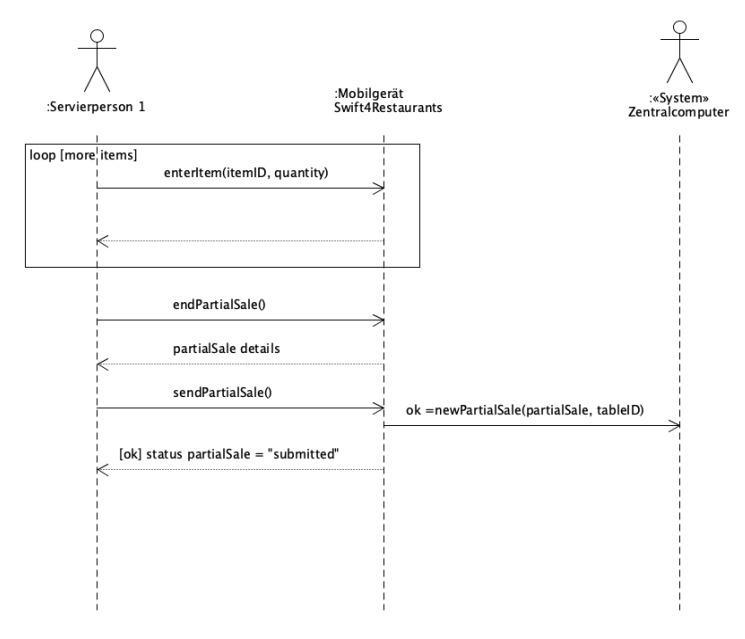
\includegraphics[width=0.3\textwidth]{Resources/Images/SSDAufgabe.png}
\caption{\label{fig:SSDAufgab}SSDAufgabe.}
\end{figure}


\subsection{Contracts}

Für die wichtigste System-Operation einen Vertrag: \\

\subparagraph{Vertrag enterItem \\}

\begin{itemize}
	\item Operation: enterItem(itemID: idemID, quantity: integer)
	\item Querverweis: UC Teilbestellung erfassen
	\item Vorbedingung: Eine Teilbestellung ist aktiv für diesen Tisch
	\item Nachbedingungen:
	\begin{itemize}
		\item bpi wurde erstellt (Bestellpositionsinstanz)
		\item bpi mit aktueller Teilbestellung für aktiven Tisch verknüpft
		\item bpi.quantity wurde auf quantity gesetzt
		\item bpi wurde anhand übereinstimmenden itemID mit einer ProductDescription verknüpft 
	\end{itemize}
\end{itemize}




\section{LE04}


\subsection{Domänenmodell Erweiterungen}

\title{Ursprüngliches Modell:}
\begin{figure}[H]
\centering
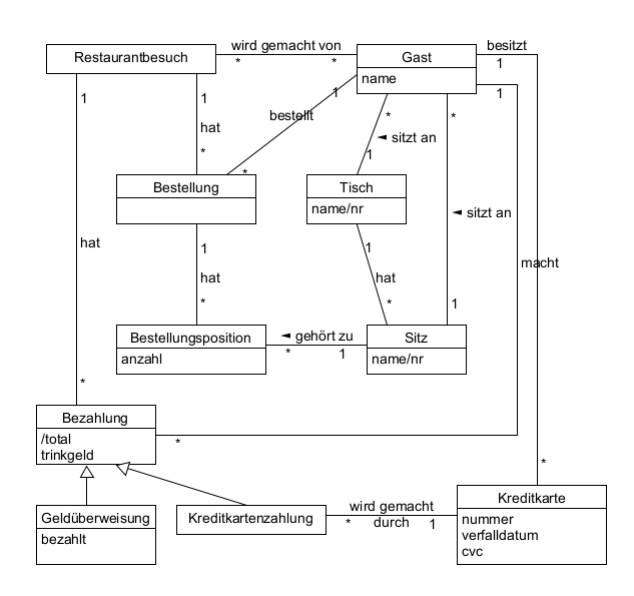
\includegraphics[width=0.3\textwidth]{Resources/Images/DMAufgabeUrsprung.png}
\caption{\label{fig:DMAufgabeUrsprung}DMAufgabeUrsprung.}
\end{figure}

\title{Verbesserungen: \\}
\begin{figure}[H]
\centering
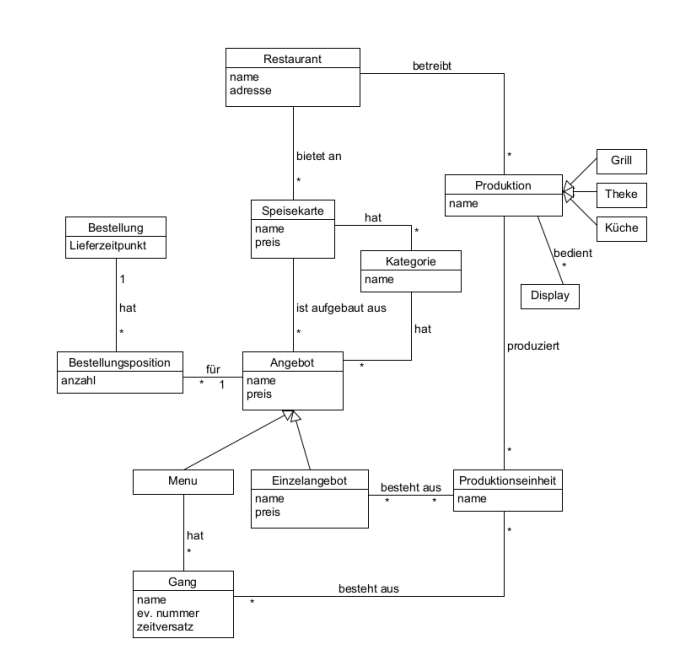
\includegraphics[width=0.3\textwidth]{Resources/Images/DMAufgabeVerbesserung.png}
\caption{\label{fig:DMAufgabeVerbesserung}DMAufgabeVerbesserung.}
\end{figure}

\begin{itemize}
	\item Produktion eingeführt als Generalisierung für mehrere Theken und Küchen
	\item Kategorien
	\item Gang (Produktionseinheit und Menu)
	\item Restaurantbesuch, zeitlich limitiert
	\item Bestellungen und Bezahlungen spezialisiert
	\item Konzept Platz eingeführt und mit Tisch verknüpft und mit Gast verbunden und mit Bestellungsposition.
\end{itemize}












































































































































































































































































\end{document}